\chapter{Simulation des robots}
	
	\section{Introduction}

		L'environnement dans lequel doivent évoluer les robots à été défini dans le \textsc{Chapitre}~\ref{chapitre:environnement}. Il est maintenant temps de simuler les \gls{ROV}s. Pour ce faire, nous allons devoir décrire les paramètres mécaniques des robots \gls{Argos} et \gls{Atoll}, ainsi que leurs capteurs et actionneurs à simuler.

	\section{Simulation des composants}
		En remarquant que les deux robots embarquent un certain nombre d'éléments communs, il est possible de definir et de simuler les différents composants dans \gls{Gazebo}, afin d'être par la suite chargés dans la simulation des deux robots. La \textsc{table}~\ref{table:components} présente les différents composants à simuler, s'ils nécéssitent l'utilisation d'un \gls{Plugin}, d'une \gls{HardwareInterface} et indique les dépendances entre les robots et ces composants.

		\begin{table}[!htb]
			\centering
			\begin{adjustbox}{max width=\textwidth}
				\begin{tabular}{|l|l|c|c|c|c|}
					\hline
					Composant & Description & \gls{Argos} & \gls{Atoll} & \gls{HardwareInterface} & \gls{Gazebo} \gls{Plugin} \\
					\hline
					\gls{Argos} Frame & Chassis d'\gls{Argos} & \cmark & \xmark & \xmark & \xmark \\
					\hline
					\gls{Atoll} Frame & Chassis d'\gls{Atoll} & \xmark & \cmark & \xmark & \xmark \\
					\hline
					Electronic Pod & Boîtier electronique & \cmark & \cmark & \xmark & \xmark \\
					\hline
					\gls{Latch} & Crochet de levage & \xmark & \cmark & \cmark & \cmark \\
					\hline
					\gls{Navcam} & Caméra de navigation & \cmark & \cmark & \xmark & \cmark \\
					\hline
					\gls{Obscam} & Caméra d'observation & \cmark & \cmark & \xmark & \cmark \\
					\hline
					Rovins & Centrale Inertielle & \cmark & \cmark & \xmark & \cmark \\
					\hline
					Spotlight & Lumières étanches & \cmark & \cmark  & \cmark & \cmark \\
					\hline
					SPE75 Thruster & Propulseur & \cmark & \cmark & \cmark & \cmark \\
					\hline
					SS309 Tilt & Nacelle pour caméra & \cmark & \cmark & \cmark & \cmark \\
					\hline
				\end{tabular}}
			\end{adjustbox}
			\caption{Composants à simuler}
			\label{table:components}
		\end{table}

		Chaque composant a ainsi un \gls{Package} de description qui lui est associe nommé suivant la convention de nommage \gls{ROS} : \textit{component\_description}. Ce package contient tout le code nécéssaire à la description du composant, c'est à dire un modèle \gls{Gazebo} permettant de simuler le composant dans le logiciel de simulation, un fichier de lancement qui s'occupe de lancer le composant dans le simulateur, les \gls{Mesh CAO}. Le code source d'un \gls{Plugin} permettant de décrire le comportement du capteur ou de l'actionneur associé au composant se trouve dans le package \textit{component\_model\_plugin}.

		Nous allons à présent détailler l'implémentation de certains composants qui ont un comportement intéressant à développer.

		\subsection{Latch}

			\subsubsection{Présentation}

				Le Latch est un composant propre au robot \gls{Atoll}. Ce crochet de levage permettant de transporter des structures sous-marines pouvant peser jusqu'à $1,5\ T$ est fabriqué par Forssea Robotics, et permet de positionner et de transporter des balises de positionnement acoustique sur les fonds marins.

			\subsubsection{Hardware Interface}


				
			\subsubsection{Model Plugin}
			
				Un \textit{Model Plugin} a été développé afin de décrire le comportement du \textit{Latch} dans \gls{Gazebo}. Il est basé sur la machine à états finis présenté en \textsc{Figure}~\ref{fig:latch_fsm} et crée un \gls{Joint} entre le \textit{Latch} et la structure à soulever de type encastrement. Les deux solides sont donc attachés l'un à l'autre jusqu'au moment où le signal de relâchement est envoyé au \textit{Latch} simulé, et le \gls{Joint} est alors supprimé.

				\begin{figure}[!htb]
					\centering
					\includegraphics[scale=0.8]{imgs/latch_fsm.pdf}
					\caption{Machine à états du \textit{Latch}}
					\label{fig:latch_fsm}
				\end{figure}

			\subsubsection{Résultats}

				On obtient alors le composant simulable dans l'environnement de simulation \gls{Gazebo}, comme on peut voir sur la \textsc{Figure}~\ref{fig:latch_gazebo}.

		\subsection{SS309 Tilt}

			\subsubsection{Présentation}

				Le \textit{SS309 Tilt} est un composant commercialisé par l'entreprise \textit{Sidus Solutions} et qui permet dans les \gls{ROV}s d'orienter l'\gls{Obscam}. Il est parfaitement étanche et comporte un jeu d'engrenages reliés à un moteur pas-à-pas pilotable en vitesse et en position. On demande ainsi au moteur de mettre l'axe à une certaine position, et l'axe se déplace avec une vitesse de rotation spécifiée.
			
			\subsubsection{Hardware Interface}

			\subsubsection{Model Plugin}

				Pour simuler cet aspect pilotable en vitesse de rotation et position, il faut passer par la simulation d'un moteur pas-à-pas. C'est un moteur un moteur composé de plusieurs bobinages créant ainsi plusieurs phases qui sont allumées succéssivement afin de réaliser une rotation de l'arbre moteur d'un certain incrément d'angle. Cet angle est défini par les caractéristiques du bobinage et n'est donc pas réglable. Il n'est pas non plus possible de piloter précisement la vitesse avec laquelle il se rend à cette position incrémentée. En revanche, il est tout à fait possible de connaître précisement la position du moteur, car l'arbre moteur ne peut prendre qu'un nombre fini d'angles, et il suffit donc de compter le nombre d'incréments commandés. Enfin, on peut commander la vitesse avec laquelle le moteur se rend à cette position, en allumant les phases à la vitesse désirée.

				Nous allons à présent distinguer la position réelle de l'arbre moteur, la position cible et la position commandée. La position réelle est la position de l'arbre moteur dans le simulateur. La position cible est un multiple de l'incrément d'angle à laquelle doit se rendre le moteur à l'instant actuel. La position commandée la position finale dans laquelle doit se retrouver l'arbre moteur et peut être une position réelle quelconque. Le moteur ne sera capable que de se rendre à la position multiple de la valeur de l'incrément d'angle la plus proche de la position commandée. La \textsc{Figure}~\ref{fig:tilt_position} reprends ces différentes notions. En commandant la vitesse à laquelle on incrémente la position cible, on contrôle l'axe en vitesse.

				\begin{figure}[!htb]
					\centering
					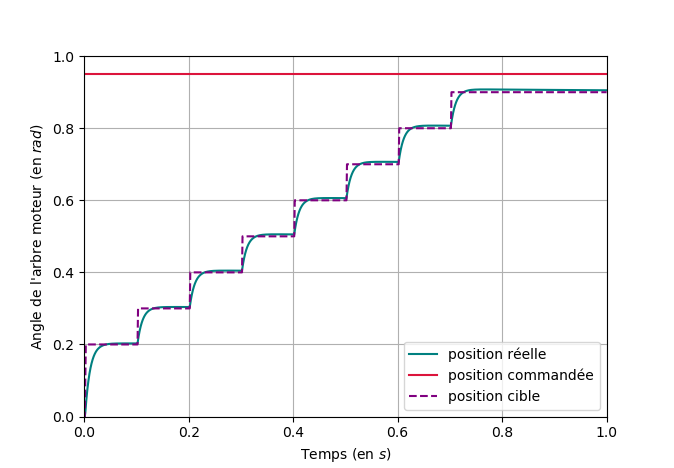
\includegraphics[width=0.6\textwidth]{imgs/stepper_motor.png}
					\caption{Simulation d'un moteur pas-à-pas}
					\label{fig:tilt_position}
				\end{figure}
				
				Pour ce qui est de l'implémentation de ce comportement dans \gls{Gazebo}, on crée un \textit{Thread} qui va s'executer en boucle avec une vitesse variable. Cette vitesse sera fonction de la vitesse de commande du \textit{Tilt} notée $\omega_c$. A chaque tour de boucle, on incrémente donc la position cible de la valeur de l'incrément $d\theta$ si la différence entre la position réelle et la position commandée est plus grande que ce même incrément, et on attends le temps $h$, avec :

				$$h = \frac{d\theta}{\omega_c}$$

				\begin{algorithm}[!htb]
					\caption{Algorithme de simulation d'un moteur pas-à-pas}
					\label{algo:stepper_motor}
					\begin{algorithmic}
						\WHILE {true}
							\STATE read $\theta_r$, $\omega_c$
							\IF {$|\theta_c - \theta_r| > d\theta$}
								\STATE $\theta_t \leftarrow \theta_t + d\theta$
							\ENDIF
							\STATE $h \leftarrow \frac{d\theta}{\omega_c}$
							\STATE sleep $h$
						\ENDWHILE
					\end{algorithmic}
				\end{algorithm}
				

	\section{Simulation d'Argos}

	\section{Simulation d'Atoll}